\section{System Design and Implementation}

\begin{figure}
    \centering
    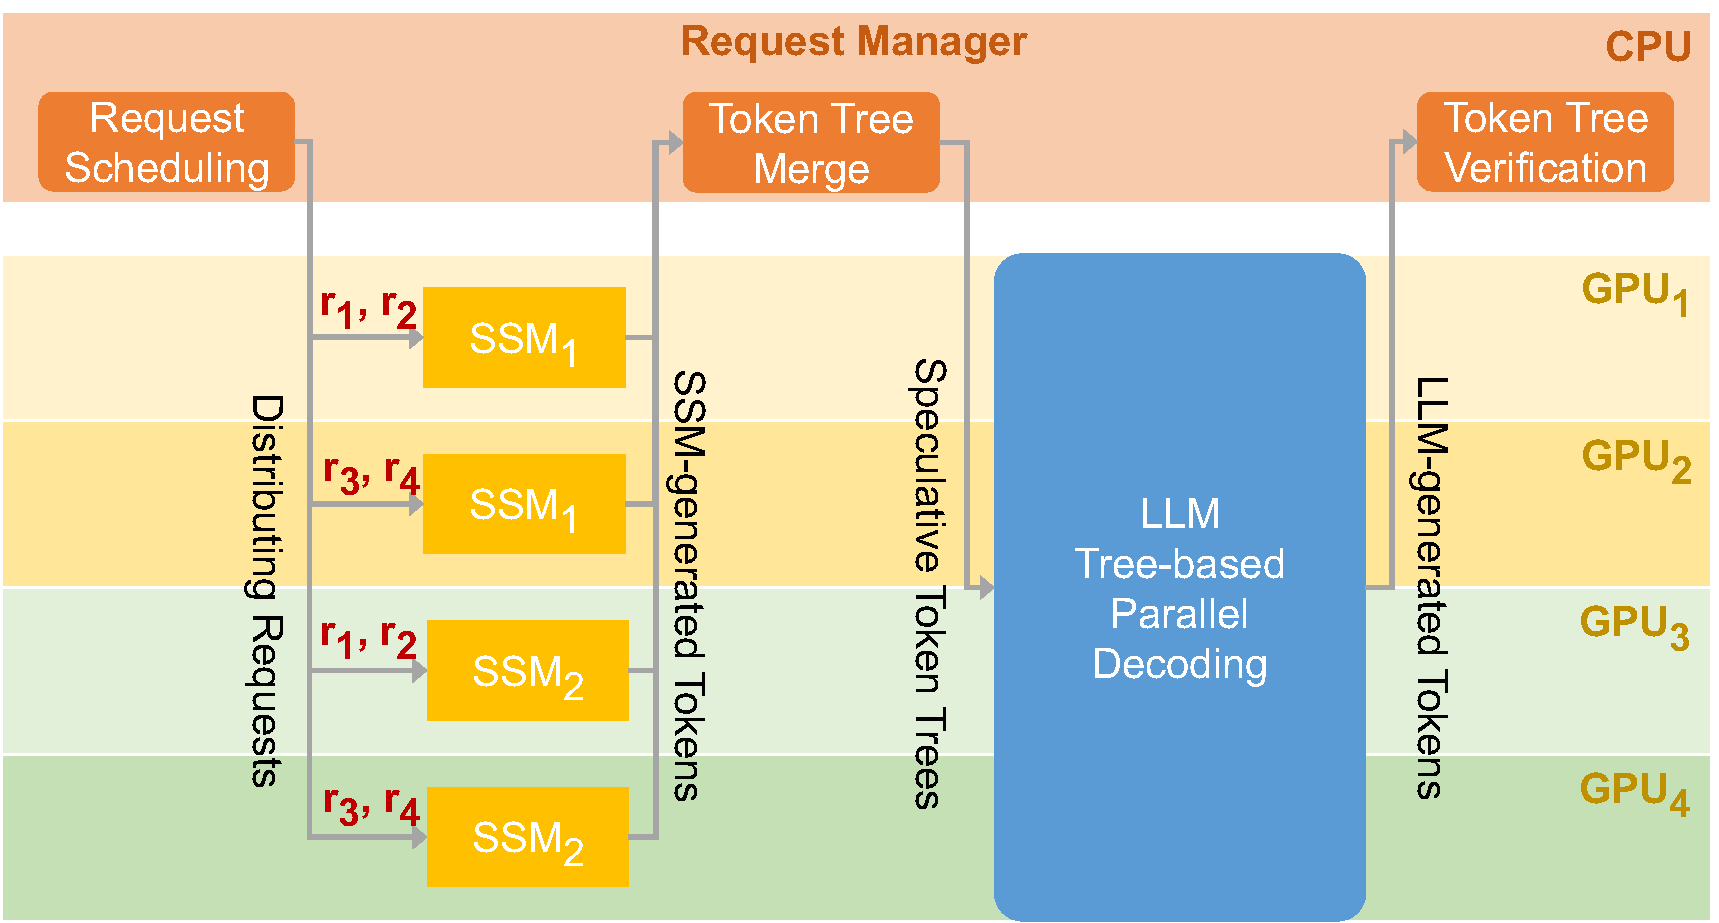
\includegraphics[scale=0.28]{figs/workflow.pdf}
    \caption{\Sys's workflow for one iteration of speculative inference and verification. \Sys uses data parallelism to serve SSMs, and combine tensor model parallelism and pipeline model parallelism for serving an LLM.}
    \label{fig:workflow}
\end{figure}

This section describes the design and implementation of \Sys's distributed runtime system (\S\ref{subsec:design} and \S\ref{subsec:implementation}), analyzes the computation and memory overheads of speculation and verification (\S\ref{subsec:overhead}), and introduces potential LLM applications that can benefit from \Sys's techniques (\S\ref{subsec:application}).

\subsection{\Sys's Runtime Design}
\label{subsec:design}
\Cref{fig:workflow} shows the workflow for one iteration of speculative inference and verification.
%%%
\Sys's {\em request manager} receives LLM serving requests and schedules these requests for serving by adapting the {\em iteration-level scheduling} policy from Orca~\cite{yu2022orca}. Specifically, \Sys iteratively selects requests from a pool of pending requests and performs one iteration of speculative inference and token tree verification for the selected requests. Since SSMs are small and can fit in one GPU, \Sys equally distributes GPUs across SSMs and serves these SSMs using data parallelism. 
For example, \Cref{fig:workflow} shows how \Sys serves two SSMs and four requests (i.e., $r_1$, $r_2$, $r_3$, and $r_4$) on four GPUs.
%%%
The SSM-generated tokens are sent back to the request manager, which produces a speculated token tree for each request using the tree merge algorithm introduced in \S\ref{sec:verification}.

\Sys serves an LLM using the hybrid parallelization strategy introduced in Megatron-LM~\cite{shoeybi2020megatronlm}, which uses tensor model parallelism for parallelizing each Transformer layer across GPUs within a node, and uses pipeline model parallelism for partitioning Transformer layers across nodes. 
All GPUs perform the tree-based parallel decoding (see \S\ref{subsec:optimization}) to compute tree attention scores and send the LLM-generated tokens back to the request manager, which finally verifies the speculated tokens against the LLM's output (see \S\ref{subsec:verification}). 

Note that the overhead introduced by the request manager (i.e., request scheduling, token tree merge, and verification) is negligible compared to the execution time of LLM inference. In addition, \sys's request manager and GPU workers only communicate tokens and do not transfer the vector representations of these tokens, which again introduces negligible communication overheads.

%\vspace{-4mm}

\paragraph{Continuous batching.}
\Sys uses {\em continuous batching} introduced in Orca~\cite{yu2022orca} to serve multiple LLM inference requests in parallel. Specifically, \sys schedules LLM execution at the granularity of iterations instead of requests. After each LLM decoding iteration, \sys checks each request's status and sends the generated results of all finished requests to the client. This design also allows \sys to start processing newly arrived requests without waiting for all current requests to complete.

\subsection{\Sys's Implementation}
\label{subsec:implementation}
\Sys was implemented on top of FlexFlow~\cite{jia2019flexflow, unger2022unity}, a distributed multi-GPU runtime for DNN computation. FlexFlow exposes an API that allows users to define a DNN model in terms of its layers.
\rev{It is compatible with PyTorch’s model definition due to the alignment of underlying operators. For example, the open-source LLMs from HuggingFace~\cite{huggingface} can be directly imported into \sys for serving without modification.}
Users can also provide a parallelization strategy, specifying the degree of data, model, and pipeline parallelism for each layer. 
%During the training phase, FlexFlow can automatically discover the best parallelization plan, which can then be saved and reused in the inference stage. 
%
A DNN is represented as a computational graph where each node is a region of memory, and each edge is an operation on one or more regions. Operations can be represented using three levels of abstraction: layers, operators, and tasks. The FlexFlow compiler transforms the computational graph from the highest abstractions (i.e., layers) to the lowest (i.e., tasks). Tasks are also the unit of parallelization; they are non-preemptible, and are executed asynchronously. 

\rev{
\paragraph{CUDA kernel optimizations.}
Directly launching cuBLAS and cuDNN kernels for calculating attention results in high kernel launch overhead and does not leverage the shared memory available on modern GPUs. To address this inefficiency, \Sys uses a customized kernel built on top of FasterTransformer~\cite{fastertransformer} for computing attention.
Within this kernel, each thread block computes a single head for a single request. The process begins with loading the query tensor into GPU shared memory accessible by all threads within a thread block. Each thread then performs a segment of the query/key product and broadcasts the result to other threads for computing the max query/key product and exponential sum.
To support tree-based parallel decoding, \sys computes all tokens within a tree in parallel and leverages the topology-aware causal mask to preserve casuality.}

\if 0
In the standard implementation of the attention mechanism, the computation of Q, K, V (Query, Key, Value) matrices and their subsequent output projection are typically consolidated within a single {\tt cublasGemmEx} function. Therefore, our optimization efforts are primarily directed toward the attention score computation phase. A challenge arises when dealing with multiple heads in the transformer architecture; the requirement to segment each head prevents the amalgamation of computations across different requests into a single operation. Consequently, conventional methods often incorporate an additional loop, where each iteration processes a singular request. This process encompasses two {\tt cublasBatchedGemm} operations and a softmax function. However, this approach introduces substantial kernel launch overhead, particularly noticeable when handling large batch sizes. To address this inefficiency, we developed a custom kernel specifically for the attention score computation, circumventing the constraints inherent to the cuBLAS API and consequently enhancing overall performance. This kernel is modified from FasterTransformer~\cite{fastertransformer}. Within our custom kernel, each thread block is assigned the task of computing a single head for a specific request. The process begins with loading the Query into shared memory, accessible by all threads within the block.  Then the kernel allocates multiple threads to each key based on predefined configurations and performs a segment of the QK product. Subsequently, these partial values are broadcast to other threads for the computation of the max QK product and the exponential sum, which are used in the softmax calculation. In addition, our custom kernel supports the Tree-based Parallel Decoding mentioned in Section 4.2. For decoding sequences in tree structures, we load all keys and values at once. This allows for the calculation of the product between all query tokens (nodes) and each key/value. If a key/value token is positioned before the root node of the tree, we retain the QK product. When the key/value is part of the tree, we consult the topology-aware causal mask to determine its relevance to the query token. If they are not relevant, the QK product is set to zero. This customization in our kernel significantly reduces launch overhead and maximizes GPU resource utilization.
\fi

\subsection{Overhead of Speculation and Verification}
\label{subsec:overhead}
\Sys accelerates generative LLM inference at the cost of additional memory and computation overheads. This section analyzes these overheads and shows that they are generally one or two orders of magnitude smaller than the memory and computation cost of executing LLM inference.

\paragraph{Memory overhead.} The memory overhead of \Sys's speculation-verification approach comes from two aspects. First, in addition to serving an LLM, \Sys also needs to allocate memory for saving the parameters of one or multiple SSMs, which collectively speculate the LLM's output. 
Our evaluation shows that \Sys can achieve significant performance improvement by using SSMs 100-1000$\times$ smaller than the LLM. As a result, hosting each SSM increases the overall memory requirement by less than 1\%. 
A second source of memory overhead comes from the token tree verification engine, which verifies an entire token tree instead of decoding a single token. 
%%%
Therefore, additional memory is needed for caching the keys and values, and storing the attention scores for all tokens. 
%%%
Due to the necessity for supporting very long sequence length in today's LLM serving, we observe that the memory overhead associated with token tree is negligible compared to key-value cache.
%%%
%For example, GPT-4 supports processing up to 32K tokens in a single request; our evaluation shows that a token tree of size 40 already allows \Sys to match 3.7 tokens on average.

\paragraph{Computation overhead.} Similarly, the computation overhead introduced by speculation and verification also comes from two aspects.
%%%
First, \Sys needs to run SSMs in the incremental-decoding mode to generate candidate tokens. When multiple SSMs are employed, \sys processes these SSMs in parallel across GPUs to minimize speculation latency.
%\Sys processes the SSMs in parallel across GPUs to minimize the latency for generating a speculated token tree.  \XM{TODO: update}
%Our evaluation shows that the latency of running a SSM in the incremental-decoding mode is 3.7$\times$ better than that of an LLM.
%%%
Second, \Sys verifies a token tree by computing the attention outputs for an entire token tree, most of which do not match the LLM's output and therefore are unnecessary in the incremental-decoding inference.
%%%
However, the key-value cache mechanism of existing LLM inference systems prevents them from serving a large number of requests in parallel, resulting in under-utilized computation resources on GPUs when serving LLMs in incremental decoding. \Sys's token tree verification leverages these under-utilized resources and therefore introduces negligible runtime overhead compared to incremental decoding.

\subsection{Applications}
\label{subsec:application}
Our speculative inference and token tree verification techniques can be directly applied to a variety of LLM applications. We identify two practical scenarios where LLM inference can significantly benefit from our techniques.

\paragraph{Distributed LLM inference.} 
The memory requirements of modern LLMs exceed the capacity of a single compute node with one or multiple GPUs, and the current approach to addressing the high memory requirement is distributing the LLM's parameters across multiple GPUs~\cite{miao2023spotserve}.
For example, serving a single inference pipeline for GPT-3 with 175 billion parameters requires more than 16 NVIDIA A100-40GB GPUs to store the model parameters in single-precision floating points.
%%%
Distributed LLM inference is largely limited by the latency to transfer intermediate activations between GPUs for each LLM decoding step. 
%%%
While \Sys's approach does not directly reduce the amount of inter-GPU communications, its verification mechanism can increase the communication granularity and reduce the number of decoding steps.


\paragraph{Offloading-based LLM inference.}
Another practical scenario that can benefit from \Sys's techniques is offloading-based LLM inference, which leverages 
CPU DRAM to store an LLM's parameters and loads a subset of these parameters to GPUs for computation in a pipeline fashion~\cite{sheng2023highthroughput}.
%%%
By opportunistically verifying multiple tokens, \Sys can reduce the number of LLM decoding steps and the overall communication between CPU DRAM and GPU HBM.